
Air resistance or drag makes ideal problems more applicable to real life. Drag consists of two terms: $f_{lin} = bv$ and $f_{quad} = cv^2$. The first linear term is proportional to the viscosity of the medium and the linear size of the object. For instance, a ball moving through molasses would have a larger $f_{lin}$ term. On the other hand, $f_{quad}$ is conceived by the fact that the object has to accelerate through the medium in which it is constantly colliding with. Most projectile drag (cannonball, etc) fall under this category, but both are shown here.

Another, more obscure way to describe each drag term is by the {\bfseries Reynold's Number}. The Reynold's number is inversely proportional to the viscosity of the medium, thus the molasses example would give intuition towards a smaller Reynold's number, that is molasses has a high viscosity. Conversely, $f_{quad}$ has a higher Reynold's number.

\begin{figure}[h]
    \centering
    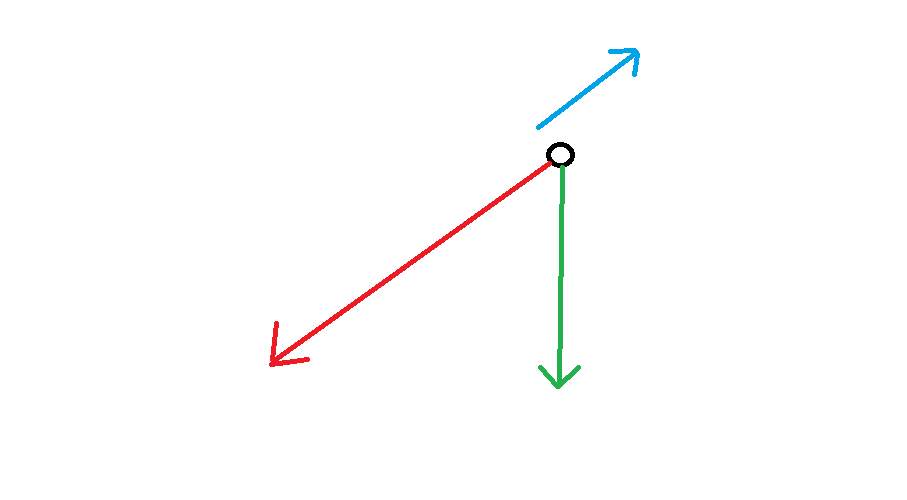
\includegraphics[width=10cm]{Classical_Mechanics/2.3-projectiles/projectile-simple.png}
    \caption{The red arrow shows drag, green shows the force due to gravity, and blue arrow shows the velocity of the object.}
    \label{fig:simple-projectile}
\end{figure}

Looking closer at linear air resistance, Newton's 2nd law becomes $m \dot v = -b v + mg$ as seen in figure \ref{fig:simple-projectile}. This is a first order differential equation for $v$, which can be solved quite handily. Breaking this equation into the components,

\begin{align}
    \label{eqn:projectile-simple-x}
    m\dot v_x = -b v_x \\
    \label{eqn:projectile-simple-y}
    m\dot v_y + b v_y = mg
\end{align}

First, we can solve equation \ref{eqn:projectile-simple-x} by integration.

\begin{equation}
    \label{eqn:projectile-simple2-x}
    \dot v_x = -\frac{b}{m}v_x
\end{equation}

\noindent By inspection, this solution must be $v_x(t) = Ae^{-\frac{b}{m}t}$, where we can replace $\frac{b}{m}$ with $\tau$ (only for linear drag). The constant $A$ is the starting velocity $v_{x0}$ when $t=0$. This makes the solution to equation \ref{eqn:projectile-simple2-x},

\begin{equation}
\label{eqn:projectile-simple3-x}
    \int_0^t v_x(t) dt = x(t) - x(0) \rightarrow x(t) = x(0) + \int^t_0 v_{x0}e^{-t/\tau} dt \rightarrow 0 + [-v_{x0} \tau e^{-t/\tau} dt] \rightarrow x_\infty(1-e^{-t/\tau}).
\end{equation}

Equation \ref{eqn:projectile-simple3-x} assumes that $x=0$ at $t=0$ and introduces a new parameter $X_\infty = v_{x0}\tau$ which is the limit of $x(t)$ at $t \rightarrow \infty$.

Taking a closer look at the y-component, for instance a projectile thrown downward. Rewriting our previous equation \ref{eqn:projectile-simple-y},

\begin{equation}
    \label{eqn:projectile-simple2-y}
    m\dot v_y = -b(v_y - v_T), v_T = \frac{mg}{b}.
\end{equation}

Equation \ref{eqn:projectile-simple2-y} introduces $v_T$, the terminal speed of an object. This is where the drag force is equal to the force by gravity, that is, the right hand side of equation \ref{eqn:projectile-simple2-y} set equal to $0$. To solve this equation, replace $v_y - v_T$ with $u$, then it becomes an equation similar to that of equation \ref{eqn:projectile-simple-x}. Solving with similar methods yields,

\begin{equation}
    \label{eqn:projectile-simple3-y}
    v_y(t) = v_T + (v_{y0} - v_T)e^{-t/\tau}.
\end{equation}

When the projectile is dropped from rest, equation \ref{eqn:projectile-simple3-y} becomes, $v_T(1-e^{-t/\tau})$. The characteristic time is useful to determine how long a falling object will take in order to reach terminal velocity. At $3\tau$, the object has reached 95\% terminal velocity. For example, oil with $v_T = \num{6.1e-5}m/s$  can be converted to $\tau$ by dividing by $g$. The oil's characteristic time $\tau = \num{6.2e-6}$. This means the oil will reach it's terminal velocity in $3\tau \approx 20$ microseconds.

